\documentclass[10pt,aspectratio=169]{beamer}
\usepackage{../../common/foundationsmacro-beamer}
\usepackage{pgfplots}
\pgfplotsset{compat=1.18}
\usepgfplotslibrary{fillbetween}
\usepackage{tikz}
\usetikzlibrary{calc,arrows.meta,decorations.pathreplacing,patterns,shapes,positioning,intersections,math,backgrounds,plotmarks,matrix}
\usepackage{booktabs}
\usepackage{bm} % For bold math symbols

% Preserve the original diagram color name using the shared course palette.
\colorlet{TitleBlue}{MacroBlue}
% Make the math letter `l` typeset as `\ell`
\AtBeginDocument{%
    \mathcode`l="8000 % make `l` active in math
    \begingroup\lccode`\~=`\l%
    \lowercase{\endgroup\def~}{\ell}% define active `l` to expand to \ell
}


% -----------------------------------------------------------------------------
% -- Title page and outline options ---- --------------------------------------
% -----------------------------------------------------------------------------

\title[Work and Leisure]{Chapter IV: Work and Leisure}

\author[Bueren]{Jes\'{u}s Bueren}

\institute{}

\date{}


%%%%%%%%%%%%%%%%%%%%%%%%%%%%%%%%%%%%%%%%%%%%%%%%%%%%%%




%%%%%%%%%%%%%%%%%%%%%%%%%%%%%%%%%%%%%%%%%%%%%%%%%%%%%%%%%%%%%%%%%%%%%%%%
\definecolor{darkgreen}{rgb}{0.0, 0.5, 0.0}
\definecolor{lightblue}{rgb}{0.3, 0.5, 0.55}
\definecolor{lightblue}{rgb}{0.3, 0.5, 0.55}
\definecolor{colormodel}{rgb}{0.3, 0.5, 0.55}

% Shared styles for the equilibrium and productivity diagrams.
\tikzset{
    prodOldDemand/.style={red!70!black,thick,dashed},
    prodNewDemand/.style={MacroBlue,very thick},
    prodSupply/.style={darkgreen,very thick},
    prodGuide/.style={gray,densely dotted},
    prodChange/.style={->,>=stealth,MacroBlue,thick}
}


\begin{document}
\begin{frame}[plain]
    \titlepage
\end{frame}


\begin{frame}{Work and Leisure: Why It Matters}

\begin{itemize}
    \item In chapter II we assumed that people worked a fixed amount ($L^s=\bar{L}$).  
    \itemvso Real life: people choose how much to work.
    \itemvso Work and leisure are important because:
    \begin{itemize}
        \itemvso Choosing a job or career is one of the biggest decisions we make.
        \itemvso The news always talks about jobs.
        \itemvso Unemployment is stressful and risky.
        \itemvso Even with a job, working more is not always better.
        \itemvso Work lets people get what they want, but it takes time away from enjoying life.
    \end{itemize}
    \itemvso How much should people work?
\end{itemize}

\end{frame}

\begin{frame}{A Simple Model of Choice}

\begin{itemize}
\item At this stage of the course, you know that we want to undertand how people choose through the lens of a model.
\itemvso The model is going to be useful to understand the key forces at play.
\itemvso In this chapter, we use a basic choice model:
\begin{itemize}
    \itemvso People have preferences over consumption and leisure.
    \itemvso Represent preferences with a utility function.
    \itemvso People pick what gives the highest utility.
    \itemvso Choices are limited by their resources (income, time).
\end{itemize}
\itemvso Household utility function:
\[
U(c, l)
\]
where $c$ is consumption and $l$ is leisure.
\end{itemize}

\end{frame}

\begin{frame}{Preferences over Consumption and Leisure}
\begin{itemize}
\item For simplicity, assume separable utility:
\[
U(c) + V(l)
\]
\vspace{-0.6cm}
\begin{itemize}
    \item $U(c)$ is happiness from consuming good.
    \itemvso $V( l )$ is happiness from leisure.
\end{itemize}
\itemvso This cannot capture the fact that some consumption activities require time (e.g., going to the movies), but it is a good starting point. 
\end{itemize}
\end{frame}


\begin{frame}{Utility Function Properties}

\begin{itemize}
\item Households like consumption:
\[
U'(c) > 0
\]
\vspace{-0.5cm}
\item Extra consumption is less valuable when you have more:
\[
U''(c) < 0
\]
\vspace{-0.5cm}
\item Households like leisure:
\[
V'(l) > 0
\]
\vspace{-0.5cm}
\item Extra leisure is less valuable the more you have:
\[
V''(l) < 0
\]
\vspace{-0.5cm}
\item Example: one hour surfing feels amazing; the fifth is not as exciting.
\end{itemize}

\end{frame}

\begin{frame}{Preferences over Consumption and Leisure}
\begin{center}
\begin{tikzpicture}
    \begin{axis}[
        axis lines=left,
        xlabel={$l$},
        ylabel={$c$},
        xlabel style={font=\small\itshape, at={(axis description cs:1.02,0)}, anchor=west},
        ylabel style={font=\small\itshape, at={(axis description cs:0,1.02)}, anchor=south, rotate=-90},
        xmin=0, xmax=1.05,
        ymin=0, ymax=14,
        width=10cm,
        height=7.5cm,
        samples=400,
        domain=0.04:0.98,
        xtick=\empty,
        ytick=\empty,
        axis line style={black, thin},
        clip=true,
    ]

    % U(c)=sqrt(c), V(l)=ln(l): isoquants c = (k - ln(l))^2
    % Named top-to-bottom so fill between outer two is unambiguous
    \addplot[color=blue!70!black,   line width=2pt, smooth, name path=curveHigh] {(2.0 - ln(x))^2};
    \addplot[color=blue!65!black,   line width=2pt, smooth]                      {(1.5 - ln(x))^2};
    \addplot[color=blue!60!black, line width=2pt, smooth, name path=curveLow]  {(0.4 - ln(x))^2};

    % Curve labels
    \node[font=\small\bfseries, color=blue!70!black,   right] at (axis cs:0.97, 4.2) {$U_3$};
    \node[font=\small\bfseries, color=blue!65!black,   right] at (axis cs:0.97,  2.4) {$U_2$};
    \node[font=\small\bfseries, color=blue!60!black, right] at (axis cs:0.97,  0.35) {$U_1$};

    \end{axis}
\end{tikzpicture}
\end{center}
\end{frame}

\begin{frame}{Preferences over Consumption and Leisure}
\begin{itemize}
    \itemvso Notice that indiference curves aren't straight lines.
    \itemvso That is because the slope changes as your move between different combinations of consumption and leisure.
    \itemvso The slope of the indifference curve is called the The marginal rate of substitution (MRS)
    \itemvso It measures how much consumption you are willing to give up for one more hour of leisure while keeping the same utility.
    \[
        MRS = \frac{\text{MU}_l}{\text{MU}_c} = \frac{V'(l)}{U'(c)}
    \]
\end{itemize}   
\end{frame}

% --- New slide: MRS along U_2 with tangent lines --------------------------
\begin{frame}{Preferences over Consumption and Leisure}
\begin{center}
\begin{tikzpicture}
    \begin{axis}[
        axis lines=left,
        xlabel={$l$},
        ylabel={$c$},
        xmin=0.04, xmax=0.98,
        ymin=0, ymax=14,
        width=10cm,
        height=7.5cm,
        samples=300,
        domain=0.04:0.98,
        xtick=\empty,
        ytick=\empty,
        axis line style={black, thin},
        clip=true,
    ]

    % U_2 isoquant (k = 1.5)
    \addplot[color=blue!65!black, line width=2pt, smooth] {(1.5 - ln(x))^2};

    % Helper: define four sample l values
    \pgfmathsetmacro{\ltwo}{0.20}
    \pgfmathsetmacro{\lthree}{0.40}
    \pgfmathsetmacro{\lfour}{0.70}

    % Compute c and slopes, plot points, labels, and tangents (explicit per point)

    \pgfmathsetmacro{\ctwo}{(1.5 - ln(\ltwo))^2}
    \pgfmathsetmacro{\mrstwo}{2*(1.5 - ln(\ltwo))/\ltwo}
    \pgfmathsetmacro{\slopetwo}{-2*(1.5 - ln(\ltwo))/\ltwo}
    \addplot[only marks, mark=*, black] coordinates {(\ltwo,\ctwo)};
    \addplot[gray, dashed, domain=\ltwo-0.08:\ltwo+0.08,line width=2pt, samples=2] {\ctwo + (\slopetwo)*(x - \ltwo)};
    \node[font=\small, anchor=south west] at (axis cs:\ltwo,\ctwo) {$\mathrm{MRS}\approx\pgfmathprintnumber[fixed,precision=2]{\mrstwo}$};

    \pgfmathsetmacro{\cthree}{(1.5 - ln(\lthree))^2}
    \pgfmathsetmacro{\mrsthree}{2*(1.5 - ln(\lthree))/\lthree}
    \pgfmathsetmacro{\slopethree}{-2*(1.5 - ln(\lthree))/\lthree}
    \addplot[only marks, mark=*, black] coordinates {(\lthree,\cthree)};
    \addplot[gray, dashed,line width=2pt, domain=\lthree-0.08:\lthree+0.08, samples=2] {\cthree + (\slopethree)*(x - \lthree)};
    \node[font=\small, anchor=south west] at (axis cs:\lthree,\cthree) {$\mathrm{MRS}\approx\pgfmathprintnumber[fixed,precision=2]{\mrsthree}$};

    \pgfmathsetmacro{\cfour}{(1.5 - ln(\lfour))^2}
    \pgfmathsetmacro{\mrsfour}{2*(1.5 - ln(\lfour))/\lfour}
    \pgfmathsetmacro{\slopefour}{-2*(1.5 - ln(\lfour))/\lfour}
    \addplot[only marks, mark=*, black] coordinates {(\lfour,\cfour)};
    \addplot[gray,line width=2pt, dashed, domain=\lfour-0.08:\lfour+0.08, samples=2] {\cfour + (\slopefour)*(x - \lfour)};
    \node[font=\small, anchor=south west] at (axis cs:\lfour,\cfour) {$\mathrm{MRS}\approx\pgfmathprintnumber[fixed,precision=2]{\mrsfour}$};

    % Label the isoquant
    \node[font=\small\bfseries, color=blue!65!black, right] at (axis cs:0.97,2.4) {$U_2$};

    \end{axis}
\end{tikzpicture}
\end{center}
\end{frame}

\begin{frame}{The Budget Constraint}
\begin{itemize}
\item Total time endowment is 1: hours worked \(h = 1 - l \).
\itemvso Consumption depends on work and wages:
\[
c = w (1-l)
\]
\itemvso The wage establishes how much consumption you can get for each unit of leisure you give up.
\end{itemize}
\end{frame}

\begin{frame}{Budget Constraint}
\begin{center}
\begin{tikzpicture}
    \begin{axis}[
        axis lines=middle,
        xlabel={$l$},
        ylabel={$c$},
        xlabel style={font=\small\itshape, at={(axis description cs:1.02,0)}, anchor=west},
        ylabel style={font=\small\itshape, at={(axis description cs:0,1.02)}, anchor=south, rotate=0},
        xmin=0, xmax=1.15,
        ymin=2, ymax=12.5,
        width=10cm,
        height=7.5cm,
        samples=400,
        domain=0:1,
        xtick=\empty,
        ytick=\empty,
        axis line style={black, thin},
        clip=true,
    ]

    % Budget constraint: w=8, T=2
    \addplot[color=red!80!black, line width=2pt, smooth, name path=budget] {8*(1-x) + 2};

    % Axis bottom (y=0) for fill
    \addplot[draw=none, name path=axisbottom] {0};

    % Fill feasible region (below budget) - visible translucent blue
    \addplot[draw=none, fill=TitleBlue!30, fill opacity=0.22] fill between[of=budget and axisbottom];

    % Endpoints
    \addplot[only marks, mark=*, color=red!80!black, mark size=2.5pt] coordinates {(0,10) (1,2)};
    \node[font=\small, anchor=west, color=red!80!black] at (axis cs:0.02,10) {$c=w$};
    \node[font=\small, anchor=east, color=red!80!black] at (axis cs:1.12,2.3) {$c=0$};

    % Interior point (feasible but not on frontier)
    \addplot[only marks, mark=*, black, mark size=2.5pt] coordinates {(0.5,3)};

    % Dashed guide lines through the interior point extended to axes
    % Vertical dashed from axis (y=0) up to frontier at y = 8*(1-0.5)+2 = 6
    \draw[gray, densely dashed] (axis cs:0.5,0) -- (axis cs:0.5,6);
    % Horizontal dashed from axis (x=0) to frontier at x solving 8*(1-x)+2 = 3 -> x = 7/8 = 0.875
    \draw[gray, densely dashed] (axis cs:0,3) -- (axis cs:0.875,3);

    % Marks where dashed lines meet the budget frontier
    \addplot[only marks, mark=*, color=red!80!black, mark size=2.5pt] coordinates {(0.5,6) (0.875,3)};

    % Marks where dashed lines meet the axes
    \addplot[only marks, mark=|, black, mark size=3pt] coordinates {(0.5,0) (0,3)};

    % Slope indicated as a small angle (no arrow)
    % pick a point on the budget line: at x=0.42, y = 8*(1-0.42)+2 = 6.64
        % horizontal baseline for slope label: from frontier to left (below the label)
        % right endpoint on budget at x=0.475 gives y = 8*(1-0.475)+2 = 6.2
        \draw[red!80!black, line width=0.9pt] (axis cs:0.475,6.2) -- (axis cs:0.34,6.2);
        % place the slope label slightly north-west of the horizontal baseline
        \node[font=\small, color=red!80!black] at (axis cs:0.39,6.4) {$w$};

    \end{axis}
\end{tikzpicture}
\end{center}
\end{frame}


\begin{frame}{Household Budget Constraint}
\begin{itemize}
\item Households spend what they can earn:
\[
c = w (1-l) 
\]
\vspace{-0.5cm}
\begin{itemize}
    \item Left side: consumption (spending)
    \itemvso Right side: income
    \begin{itemize}
        \itemvso Labor income: \(w (1-l)\)
    \end{itemize}
\end{itemize}
\end{itemize}

\end{frame}

% --- New slide: Budget + U_2 with intersection and MRS --------------------------



\begin{frame}{The Problem}

\begin{itemize}
\item Maximize utility by choosing leisure \(l\) and consumption \(c\):
\[
\max_{c,l} \ U(c) + V(l)
\]\\
\vspace{-0.5cm}
\item Subject to the budget constraint:
\[
c = w (1-l)
\]
\itemvso Question: how much leisure should a person enjoy to maximize happiness?
\end{itemize}

\end{frame}

\begin{frame}{Solving the Problem}

\begin{itemize}
\item Plug budget into utility:
\[
U(c) + V(l) \longrightarrow U(\underbrace{w (1-l)}_{c}) + V(l)
\]
\vspace{-0.3cm}
\item Take derivative with respect to leisure \(l\) and set to zero:
\[
\frac{d}{dl} \big[ U(\underbrace{w (1-l)}_{c}) + V(l) \big] = 0
\]
\item Using chain rule:
\[
-w U'(c) + V'(l) = 0
\]
\item Rearrange:
\[
w U'(c) = V'(l) \Leftrightarrow  MRS=\dfrac{V'(l)}{U'(c)}=w
\]
\item This equation tells us the optimal leisure (and therefore work).
\end{itemize}
\end{frame}

\begin{frame}{What the Equation Means}

\begin{itemize}
\item Optimal condition:
\[
w U'(c) = V'(l)
\]
\itemvso In plain words, working one extra hour:
\begin{itemize}
    \itemvso Brings you extra happiness from consuming what you earn for working one more hour by \(w U'(c)\)
    \itemvso But lowers your happiness from an extra hour of work by \(V'(l)\)
    \itemvso At the optimum, these are equal\\
    \vspace{0.3cm}
     the marginal gain from consumption = the marginal loss from leisure
\end{itemize}
\end{itemize}

\end{frame}


\begin{frame}{Intuition: Few Hours vs Many Hours}

\begin{itemize}
\item Very few hours worked (lots of leisure):
\begin{itemize}
    \itemvso \(U'(c)\) large (not enough income, coconuts are valuable)
    \itemvso \(V'(l)\) low (already lots of surfing)
    \itemvso Equation says: work more, surf less → increase overall happiness
\end{itemize}

\itemvso Very many hours worked (no surfing):
\begin{itemize}
    \itemvso \(U'(c)\) small (income is enough, coconuts not as valuable)
    \itemvso \(V'(l)\) large (not much surfing)
    \itemvso Equation says: work less, surf more → increase overall happiness
\end{itemize}
\end{itemize}

\end{frame}

\begin{frame}{Finding the Sweet Spot}

\begin{itemize}
\item Somewhere in the middle, optimal leisure \(l^*\) satisfies:
\[
w U'(c) = V'(l)
\]
\itemvso One more hour of work would make you less happy (loss of leisure > gain in consumption)
\itemvso One more hour of leisure would reduce consumption too much (gain in leisure $<$ loss in consumption)
\itemvso This is the household’s best choice for work and leisure.
\end{itemize}

\end{frame}

\begin{frame}{Solving the Problem}
\centering
\begin{tikzpicture}
    \begin{axis}[
        compat=1.18,
        axis lines=left,
        xlabel={$l$},
        ylabel={$c$},
        xmin=0.04, xmax=0.98,
        ymin=1.5, ymax=14,
        width=10cm,
        height=7.5cm,
        samples=200,
        domain=0.04:0.98,
        xtick=\empty,
        ytick=\empty,
        axis line style={black, thin},
        clip=true,
    ]

    % Parameters
    \pgfmathsetmacro{\w}{8}
    \pgfmathsetmacro{\T}{2}
    \pgfmathsetmacro{\kUtwo}{1.5}

    % Budget constraint and U_2 isoquant
    \addplot[color=red!80!black, line width=2pt] {\w*(1-x) + \T};
  
    \addplot[color=blue!65!black, line width=2pt, smooth] {(\kUtwo - ln(x))^2};
  \only<1>{
    % Left-hand intersection (intersection of U_2 and budget)
    \pgfmathsetmacro{\lint}{0.275}
    \pgfmathsetmacro{\cint}{(\kUtwo - ln(\lint))^2}
    \pgfmathsetmacro{\MRSint}{2*(\kUtwo - ln(\lint))/\lint}
    \pgfmathsetmacro{\mint}{-\MRSint}
    
    
    % mark the intersection point and show its MRS (this is where MRS != w)
    \addplot[only marks, mark=*, black] coordinates {(\lint,\cint)};
    \node[font=\small, anchor=south west] at (axis cs:\lint,\cint) {$\mathrm{MRS}>w$};

    % Draw a short MRS segment at the intersection point
    \pgfmathsetmacro{\d}{0.2}
    \pgfmathsetmacro{\xleft}{max(0.04,\lint-\d)}
    \pgfmathsetmacro{\xright}{min(0.98,\lint+\d)}
    \pgfmathsetmacro{\yleft}{\cint + \mint*(\xleft - \lint)}
    \pgfmathsetmacro{\yright}{\cint + \mint*(\xright - \lint)}
    \draw[black!70, dashed, line width=2pt] (axis cs:\xleft,\yleft) -- (axis cs:\xright,\yright);
    }
    % Compute isoquant tangent to budget where MRS = w (solve quadratic)
    \pgfmathsetmacro{\acoef}{(\w^2)/4}
    \pgfmathsetmacro{\bcoef}{\w}
    \pgfmathsetmacro{\ccoef}{-(\w+\T)}
    \pgfmathsetmacro{\disc}{\bcoef^2 - 4*\acoef*\ccoef}
    \pgfmathsetmacro{\ltone}{(-\bcoef + sqrt(\disc))/(2*\acoef)}
    \pgfmathsetmacro{\lttwo}{(-\bcoef - sqrt(\disc))/(2*\acoef)}
    \pgfmathsetmacro{\lt}{ifthenelse(\ltone>0 && \ltone<1, \ltone, \lttwo)}
    \pgfmathsetmacro{\ktang}{ln(\lt) + (\w*\lt)/2}
    \pgfmathsetmacro{\ctang}{(\ktang - ln(\lt))^2}
    
    \only<2>{
    % Plot the isoquant tangent to the budget (MRS = w)
    \addplot[color=blue!65!black, line width=2pt, smooth, domain=0.04:0.98] {(\ktang - ln(x))^2};
    \node[font=\small, color=blue!65!black, right] at (axis cs:0.6,6) {$\mathrm{MRS}=w$};

    % mark tangency point (this is the max-utility point on the budget)
    
    \addplot[only marks, mark=*, blue!65!black, mark options={fill=blue!65!black}] coordinates {(\lt,\ctang)};
    \node[font=\small, pin=45:{$(l^*,c^*)$}] at (axis cs:\lt,\ctang) {};
    }

    \end{axis}
\end{tikzpicture}
\end{frame}

\begin{frame}{Poll}

Suppose your wage was higher.  
How would this affect your labor supply?

\bigskip

\begin{itemize}
    \item I would work more
    \itemvso I would work the same amount
    \itemvso I would work less
\end{itemize}

\end{frame}

\begin{frame}{Substitution and Income Effects --- Substitution Effect Dominates}
\centering
\begin{tikzpicture}
    \begin{axis}[
        compat=1.18,
        axis lines=left,
        xlabel={$l$},
        ylabel={$c$},
        xmin=0.04, xmax=1.05,
        ymin=2, ymax=20,
        width=10cm,
        height=7.5cm,
        samples=200,
        domain=0.04:1.0,
        xtick=\empty,
        ytick=\empty,
        axis line style={black, thin},
        clip=true,
    ]

    % ---------- Parameters (all pre-solved in Python) ----------
    \pgfmathsetmacro{\wlow}{6}
    \pgfmathsetmacro{\whigh}{12}
    \pgfmathsetmacro{\T}{2}

    % Original optimum A (low wage, w=6)
    \pgfmathsetmacro{\ltL}{0.666667}
    \pgfmathsetmacro{\ktangL}{1.594535}
    \pgfmathsetmacro{\ctangL}{4.000000}

    % New optimum B (high wage, w=12)
    \pgfmathsetmacro{\ltH}{0.478831}
    \pgfmathsetmacro{\ktangH}{2.136575}
    \pgfmathsetmacro{\ctangH}{8.254033}

    % Compensated Slutsky point S
    % Solves: whigh*lS/2 + ln(lS) = ktangL, same utility as A, slope = whigh
    \pgfmathsetmacro{\lS}{0.413100}
    \pgfmathsetmacro{\cS}{6.143460}
    \pgfmathsetmacro{\compInt}{11.100660}   % intercept: c = compInt - whigh*l

    % ---------- Budget constraints ----------
    % BL1: original (w=6), passes through (1, T)
    \addplot[color=red!70!black, line width=2pt] {\wlow*(1-x) + \T};
    %\node[font=\small, color=red!70!black] at (axis cs:0.08,{\wlow*0.92+\T+0.5}) {$BL_1$};

    % BL2: new (w=12), passes through (1, T)
    \addplot[color=red!40!orange, line width=2pt, dashed] {\whigh*(1-x) + \T};
    %\node[font=\small, color=red!40!orange] at (axis cs:0.08,{\whigh*0.92+\T+0.5}) {$BL_2$};

    % BL_comp: same slope as BL2, tangent to U1 at S
   \only<2>{
    \addplot[color=gray!80, line width=1.5pt, dotted] {\compInt - \whigh*x};
    }
    %\node[font=\small, color=gray!60] at (axis cs:0.65,{\compInt - \whigh*0.65 + 0.7}) {$BL^{comp}$};



    % ---------- Indifference curves ----------
    % U1: original utility (k = ktangL)
    \addplot[color=blue!65!black, line width=2pt, smooth] {(\ktangL - ln(x))^2};
    \node[font=\small, color=blue!65!black] at (axis cs:0.9,{(\ktangL-ln(0.9))^2+0.6}) {$U_1$};

    % U2: higher utility (k = ktangH)
    \addplot[color=blue!40!cyan, line width=2pt, smooth] {(\ktangH - ln(x))^2};
    \node[font=\small, color=blue!40!cyan] at (axis cs:0.9,{(\ktangH-ln(0.9))^2+0.6}) {$U_2$};

    % ---------- Optimal points ----------
    % A: original optimum
    \addplot[only marks, mark=*, blue!65!black, mark options={fill=blue!65!black}]
        coordinates {(\ltL,\ctangL)};
    \node[font=\small, anchor=south east] at (axis cs:\ltL,\ctangL) {$A$};

    % S: Slutsky compensated point (same U1, high-wage slope)
    \only<2>{
    \addplot[only marks, mark=*, gray!80!black, mark options={fill=gray!60}]
        coordinates {(\lS,\cS)};
    \node[font=\small, anchor=south east] at (axis cs:\lS,\cS) {$S$};
    % Arrows showing substitution effect (A->S) and income effect (S->B)
    \draw[->, >=stealth, thick, green!60!black]
        (axis cs:\ltL, \ctangL) .. controls (axis cs:{(\ltL+\lS)/2}, {\ctangL+1.2}) .. (axis cs:\lS, \cS);
    \node[font=\small, green!60!black, fill=white, inner sep=1pt] at (axis cs:{(\ltL+\lS)/2}, {\ctangL+1.8}) {SE};

    \draw[->, >=stealth, thick, orange!80!black]
        (axis cs:\lS, \cS) .. controls (axis cs:{(\lS+\ltH)/2}, {\cS+1.2}) .. (axis cs:\ltH, \ctangH);
    \node[font=\small, orange!80!black, fill=white, inner sep=1pt] at (axis cs:{(\lS+\ltH)/2}, {\cS+1.8}) {IE};
    }

    % B: new optimum (high wage)
    \addplot[only marks, mark=*, blue!40!cyan, mark options={fill=blue!40!cyan}]
        coordinates {(\ltH,\ctangH)};
    \node[font=\small, anchor=south west] at (axis cs:\ltH,\ctangH) {$B$};

    % ---------- Effect arrows below x-axis ----------
    % Substitution effect A->S: leisure falls (left)
    \draw[<->, >=stealth, thick, green!60!black]
        (axis cs:\lS,-1.2) -- (axis cs:\ltL,-1.2)
        node[midway, below, font=\tiny] {SE};

    % Income effect S->B: leisure rises (right) -- normal good
    \draw[<->, >=stealth, thick, orange!80!black]
        (axis cs:\lS,-1.2) -- (axis cs:\ltH,-1.2)
        node[midway, below, font=\tiny] {IE};

    % Total effect A->B: net reduction in leisure
    \draw[<->, >=stealth, thick, purple!70!black]
        (axis cs:\ltH,-2.5) -- (axis cs:\ltL,-2.5)
        node[midway, below, font=\tiny] {Total};

    \end{axis}
\end{tikzpicture}
\end{frame}


\begin{frame}{Substitution and Income Effects --- Income Effect Dominates}
\centering
\begin{tikzpicture}
    \begin{axis}[
        compat=1.18,
        axis lines=left,
        xlabel={$l$},
        ylabel={$c$},
        xmin=0.04, xmax=1.05,
        ymin=2, ymax=14,
        width=10cm,
        height=7.5cm,
        samples=200,
        domain=0.04:1.0,
        xtick=\empty,
        ytick=\empty,
        axis line style={black, thin},
        clip=true,
    ]

    % u(l,c) = sqrt(l*(c-4)),  wlow=4, whigh=8, T=2
    % Both BLs pass through (l=1, c=T=2). All points pre-solved analytically.
    \pgfmathsetmacro{\wlow}{4}
    \pgfmathsetmacro{\whigh}{8}
    \pgfmathsetmacro{\T}{2}
    \pgfmathsetmacro{\czero}{4}   % subsistence consumption

    % Point A: original optimum (w=4)
    \pgfmathsetmacro{\ltL}{0.250000}
    \pgfmathsetmacro{\ctL}{5.000000}

    % Point S: Slutsky compensated (same U1, slope = whigh=8)
    \pgfmathsetmacro{\lS}{0.176777}
    \pgfmathsetmacro{\cS}{5.414214}
    \pgfmathsetmacro{\compInt}{6.828427}   % c = compInt - whigh*l

    % Point B: new optimum (w=8)
    \pgfmathsetmacro{\ltH}{0.375000}
    \pgfmathsetmacro{\ctH}{7.000000}

    % IC constants: U1: c = czero + K1sq/l,   U2: c = czero + K2sq/l
    \pgfmathsetmacro{\Konesq}{0.250000}
    \pgfmathsetmacro{\Ktwosq}{1.125000}

    % ---------- Budget constraints ----------
    % BL1: c = 4*(1-l) + 2, passes through (1, 2)
    \addplot[color=red!70!black, line width=2pt] {\wlow*(1-x) + \T};
    %\node[font=\small, color=red!70!black] at (axis cs:0.65,{\wlow*(1-0.65)+\T+0.5}) {$BL_1$};

    % BL2: c = 8*(1-l) + 2, passes through (1, 2)
    \addplot[color=red!40!orange, line width=2pt, dashed] {\whigh*(1-x) + \T};
    %\node[font=\small, color=red!40!orange] at (axis cs:0.35,{\whigh*(1-0.35)+\T+0.5}) {$BL_2$};

    % BL_comp: c = 6.828 - 8*l (same slope as BL2, tangent to U1 at S)
    \addplot[color=gray!80, line width=1.5pt, dotted, domain=0.04:0.854] {\compInt - \whigh*x};
    %\node[font=\small, color=gray!60] at (axis cs:0.65,{\compInt - \whigh*0.65 + 0.5}) {$BL^{comp}$};

    % Common anchor point (1, T) = (1, 2)
    \addplot[only marks, mark=*, black, mark options={fill=black}] coordinates {(1,\T)};
    \node[font=\small, anchor=north west] at (axis cs:1,\T) {$T$};

    % ---------- Indifference curves ----------
    % U1: c = czero + K1sq/l
    \addplot[color=blue!65!black, line width=2pt, smooth, domain=0.04:0.95]
        {\czero + \Konesq/x};
    \node[font=\small, color=blue!65!black]
        at (axis cs:0.07,{\czero + \Konesq/0.07 + 0.4}) {$U_1$};

    % U2: c = czero + K2sq/l
    \addplot[color=blue!40!cyan, line width=2pt, smooth, domain=0.09:0.95]
        {\czero + \Ktwosq/x};
    \node[font=\small, color=blue!40!cyan]
        at (axis cs:0.12,{\czero + \Ktwosq/0.12 + 0.4}) {$U_2$};

    % ---------- Optimal points ----------
    % A
    \addplot[only marks, mark=*, blue!65!black, mark options={fill=blue!65!black}]
        coordinates {(\ltL,\ctL)};
    \node[font=\small, anchor=south east] at (axis cs:\ltL,\ctL) {$A$};

    % S
    \addplot[only marks, mark=*, gray!80!black, mark options={fill=gray!60}]
        coordinates {(\lS,\cS)};
    \node[font=\small, anchor=north east] at (axis cs:\lS,\cS) {$S$};

    % B
    \addplot[only marks, mark=*, blue!40!cyan, mark options={fill=blue!40!cyan}]
        coordinates {(\ltH,\ctH)};
    \node[font=\small, anchor=south west] at (axis cs:\ltH,\ctH) {$B$};

    % ---------- Effect arrows below x-axis ----------
    % SE: A->S (leisure falls)
    \draw[<->, >=stealth, thick, green!60!black]
        (axis cs:\lS,-1.0) -- (axis cs:\ltL,-1.0)
        node[midway, below, font=\tiny] {SE};

    % IE: S->B (leisure rises, DOMINATES)
    \draw[<->, >=stealth, thick, orange!80!black]
        (axis cs:\lS,-1.0) -- (axis cs:\ltH,-1.0)
        node[midway, below, font=\tiny] {IE};

    % Total: A->B (net leisure rises)
    \draw[<->, >=stealth, thick, purple!70!black]
        (axis cs:\ltL,-2.2) -- (axis cs:\ltH,-2.2)
        node[midway, below, font=\tiny] {Total $>0$};

    \end{axis}
\end{tikzpicture}

\end{frame}

\begin{frame}{Income vs. Substitution Effects}

With an increase in wages, the effect on labor supply depends on which force dominates:

\bigskip

\begin{itemize}
    \item Substitution effect: leisure becomes more expensive  
    $\Rightarrow$ work more
    \item Income effect:  higher income increases demand for leisure  
    $\Rightarrow$ work less
\end{itemize}

\bigskip

Depending on whether the income or the substitution effect dominates, you would work more or less.

\end{frame}

\begin{frame}{Income vs. Substitution Effects: Cross-Country Evidence}

\begin{columns}[onlytextwidth]

\begin{column}{0.44\textwidth}
\begin{itemize}
\item Bick et al.\ (2018) study labor supply responses using cross-country variation.

\itemvso There is a negative correlation between hours worked and GDP per capita, suggesting that the income effect tends to dominate. 
\itemvso The relationship is not very strong, indicating that income and substitution effects partly offset each other.
\end{itemize}
\end{column}

\begin{column}{0.53\textwidth}
\begin{figure}
    \centering
    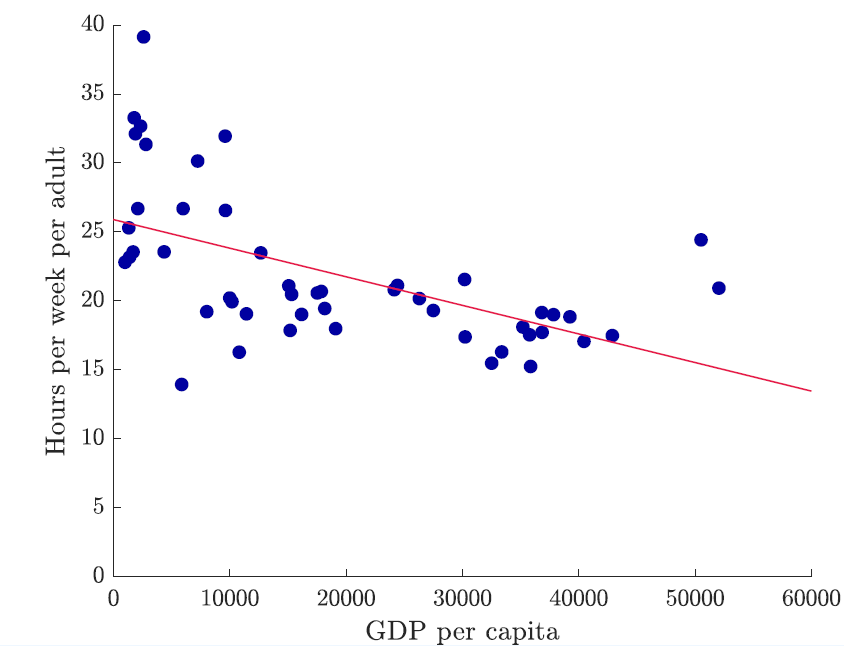
\includegraphics[width=\textwidth,height=4.8cm,keepaspectratio]{figures/inc_subs}
    \caption{\footnotesize
    Hours Worked and GDP per Capita Across Countries
    }
    \vspace{0.2cm}
    \begin{flushleft}
    \footnotesize \textit{Source:} Bick, Fuchs-Schündeln, and Lagakos (2018).
    \end{flushleft}
\end{figure}
\end{column}

\end{columns}

\end{frame}

\begin{frame}{Comparing the US and Europe}

\begin{columns}[onlytextwidth]

\begin{column}{0.44\textwidth}
\small
\begin{itemize}
\item The figure shows the evolution of hours worked per employed person in the US and Europe.

    \itemvso Until the early 1970s, the US and Western Europe looked very similar
    \itemvso After that, hours diverged
    \itemvso Today, Europeans work substantially less than Americans
\end{itemize}

\bigskip

\textbf{Why did this divergence occur?}

\end{column}

\begin{column}{0.53\textwidth}
\begin{figure}
    \centering
    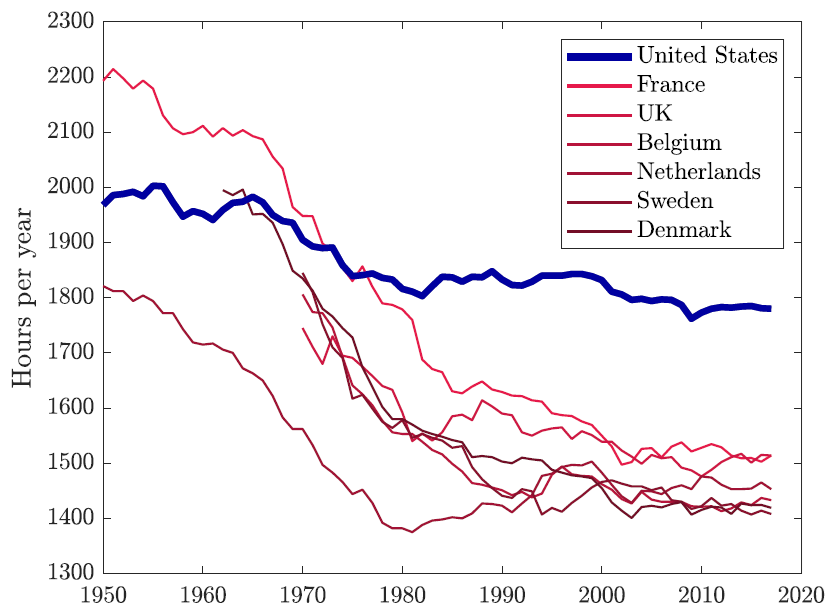
\includegraphics[width=\textwidth,height=4.8cm,keepaspectratio]{figures/us_europe_hours}
    \caption{\footnotesize
    Hours Worked per Employed Person: US vs. Europe
    }
    \vspace{0.2cm}
    \begin{flushleft}
    \footnotesize \textit{Source:} OECD
    \end{flushleft}
\end{figure}
\end{column}

\end{columns}

\end{frame}

\begin{frame}{Why Do Europeans Work Less Than Americans?}

\small
Several explanations have been proposed for the divergence in hours worked between the US and Europe:

\bigskip

\begin{itemize}
    \item \textbf{Taxes and social insurance (Prescott, 2004):}  
    Higher labor taxes and more generous social security systems in Europe reduce incentives to work.

    \medskip
    \item \textbf{Labor supply elasticity:}  
    Prescott’s explanation requires a high elasticity of labor supply, which is larger than most microeconomic estimates.

    \medskip
    \item \textbf{Timing:}  
    Policy differences emerged in the 1960s–1970s, but the divergence in hours continued to grow long after.

    \medskip
    \item \textbf{Preferences (Blanchard, 2004):}  
    Europeans may value leisure more than Americans (Economists tend to be a little bit uncomfortable with explanations based on differences in
preferences: hard to test).

    \medskip
    \item \textbf{Institutions and unions (Alesina et al., 2006):}  
    Stronger unions in Europe may lead to shorter working hours and longer holidays.
\end{itemize}

\end{frame}

\begin{frame}{Taxes, Transfers, and Labor Supply}

\begin{itemize}


\item Consider the effect of taxes and transfers on an individual's labor supply decision.

\bigskip

\textbf{Transfers:} $c=w(1-\ell) + T$
\begin{itemize}
    \item Do not change prices
    \item Make the worker richer
    \item Generate a pure income effect
\end{itemize}
\bigskip


\textbf{Taxes:} $c=w(1-\ell) (1-\tau)$
\begin{itemize}
    \item Labor income is taxed at rate $\tau$
    \item The worker receives the after-tax wage $w(1-\tau)$
    \item Taxes lower the slope of the budget constraint
\end{itemize}


\end{itemize}
\end{frame}

\begin{frame}{Transfers: Lump-sum Transfer and the Income Effect}
\begin{center}
\begin{tikzpicture}
    \begin{axis}[
        compat=1.18,
        axis lines=left,
        xlabel={$l$},
        ylabel={$c$},
        xmin=0.01, xmax=1.05,
        ymin=0, ymax=13,
        width=10cm,
        height=7.5cm,
        samples=200,
        domain=0.01:1,
        xtick=\empty,
        ytick=\empty,
        axis line style={black, thin},
        clip=true,
    ]

    % ----- Parameters -----
    \pgfmathsetmacro{\w}{8}
    \pgfmathsetmacro{\T}{2}

    % Tangency points
    \pgfmathsetmacro{\lA}{0.25}
    \pgfmathsetmacro{\cA}{6}

    \pgfmathsetmacro{\lB}{0.375}
    \pgfmathsetmacro{\cB}{7}

    % Indifference constants
    \pgfmathsetmacro{\Kone}{9}
    \pgfmathsetmacro{\Ktwo}{12.25}

    % ----- Budget constraints -----
    % BL1: c = 8(1-l)
    \addplot[color=red!70!black, line width=2pt] {\w*(1-x)};

    % BL2: c = 8(1-l)+2
    \addplot[color=red!40!orange, line width=2pt, dashed] {\w*(1-x)+\T};

    % ----- Indifference curves -----
    \addplot[color=blue!70!black, line width=2pt, smooth]
        {\Kone/(1+2*x)};
    \node[font=\small, color=blue!70!black]
        at (axis cs:0.1,8) {$U_1$};

    \addplot[color=blue!40!cyan, line width=2pt, smooth]
        {\Ktwo/(1+2*x)};
    \node[font=\small, color=blue!40!cyan]
        at (axis cs:0.2,10) {$U_2$};

    % ----- Optimal points -----
    % A
    \addplot[only marks, mark=*, blue!70!black, mark options={fill=blue!70!black}]
        coordinates {(\lA,\cA)};
    \node[font=\small, anchor=south east] at (axis cs:\lA,\cA) {$A$};

    % B
    \addplot[only marks, mark=*, blue!40!cyan, mark options={fill=blue!40!cyan}]
        coordinates {(\lB,\cB)};
    \node[font=\small, anchor=south west] at (axis cs:\lB,\cB) {$B$};

    % ----- Transfer arrow -----
    \draw[->, >=stealth, thick]
        (axis cs:1,0) -- (axis cs:1,2)
        node[midway, right, font=\small] {$T$};

    % Income Effect: S -> B
    \draw[->, >=stealth, thick, orange!80!black]
        (axis cs:\lA,\cA) -- (axis cs:\lB,\cB)
        node[midway, below, font=\tiny] {IE};

    \end{axis}
\end{tikzpicture}
\end{center}
\end{frame}

\begin{frame}{Taxes: Income and Substitution Effects}
\begin{center}
\begin{tikzpicture}
    \begin{axis}[
        compat=1.18,
        axis lines=left,
        xlabel={$l$},
        ylabel={$c$},
        xmin=0.01, xmax=1.05,
        ymin=0, ymax=13,
        width=10cm,
        height=7.5cm,
        samples=200,
        domain=0.01:1,
        xtick=\empty,
        ytick=\empty,
        axis line style={black, thin},
        clip=true,
    ]

    % ----- Parameters -----
    \pgfmathsetmacro{\wH}{8}
    \pgfmathsetmacro{\wL}{4}

    % Points
    \pgfmathsetmacro{\lA}{0.25}
    \pgfmathsetmacro{\cA}{6}

    \pgfmathsetmacro{\lB}{0.25}
    \pgfmathsetmacro{\cB}{3}

    \pgfmathsetmacro{\lS}{0.561}
    \pgfmathsetmacro{\cS}{4.243}

    % Indifference curve constants
    \pgfmathsetmacro{\Kone}{9}
    \pgfmathsetmacro{\Ktwo}{4.5}

    % Compensated budget intercept
    \pgfmathsetmacro{\compInt}{6.485}

    % ---------- Budget constraints ----------
    % BL1 (w=8)
    \addplot[color=red!70!black, line width=2pt]
        {\wH*(1-x)};

    % BL2 (w=4)
    \addplot[color=red!40!orange, line width=2pt, dashed]
        {\wL*(1-x)};

    % Compensated budget line (parallel to BL2)
    \addplot[color=gray!80, line width=1.5pt, dotted]
        {\compInt - \wL*x};

    % ---------- Indifference curves ----------
    \addplot[color=blue!65!black, line width=2pt, smooth]
        {\Kone/(1+2*x)};
    \node[font=\small, color=blue!65!black]
        at (axis cs:0.08,8.5) {$U_1$};

    \addplot[color=blue!40!cyan, line width=2pt, smooth]
        {\Ktwo/(1+2*x)};
    \node[font=\small, color=blue!40!cyan]
        at (axis cs:0.08,4.4) {$U_2$};

    % ---------- Points ----------
    % A
    \addplot[only marks, mark=*, blue!65!black, mark options={fill=blue!65!black}]
        coordinates {(\lA,\cA)};
    \node[font=\small, anchor=south east] at (axis cs:\lA,\cA) {$A$};

    % B
    \addplot[only marks, mark=*, blue!40!cyan, mark options={fill=blue!40!cyan}]
        coordinates {(\lB,\cB)};
    \node[font=\small, anchor=north east] at (axis cs:\lB,\cB) {$B$};

    % S (Slutsky point)
    \addplot[only marks, mark=*, gray!80!black, mark options={fill=gray!60}]
        coordinates {(\lS,\cS)};
    \node[font=\small, anchor=south west] at (axis cs:\lS,\cS) {$S$};
    
      % ---------- Effect arrows below x-axis ----------
    % Substitution Effect: A -> S
    \draw[->, >=stealth, thick, green!60!black]
        (axis cs:\lA,\cA) -- (axis cs:\lS,\cS)
        node[midway, above, font=\tiny] {SE};

    % Income Effect: S -> B
    \draw[->, >=stealth, thick, orange!80!black]
        (axis cs:\lS,\cS) -- (axis cs:\lB,\cB)
        node[midway, below, font=\tiny] {IE};

    \end{axis}
\end{tikzpicture}
\end{center}
\end{frame}

\begin{frame}{Equilibrium in the labor Market with elastic labor supply}
\begin{itemize}
\item Now we are going to go back to the model that we covered in chapter 2, and analyze the equilibrium when labor supply is elastic.
\itemvso The key difference is that now we allow workers to adjust their labor supply in response to changes in wages.
\itemvso Production is still Cobb-Douglas, and firms are competitive.
\itemvso Capital supply is fixed and equal to $\bar{K}$
\end{itemize}
\end{frame}

\begin{frame}{Equilibrium in the labor Market with elastic labor supply}
\begin{itemize}
    \item Labor demand is derived from the firm’s profit maximization problem:
    \[
    \max_{K,L} F(K,L) - wL - rK
    \]  
    \vspace{-0.3cm}
    \item Firms hire labor up to the point where
    \[
    w = F_L(K,L)
    \]
    \vspace{-0.3cm}
    \item This equation defines the \textbf{labor demand curve}
\itemvso The labor demand curve is downward sloping because of the diminishing marginal product of labor.
\itemvso \textbf{Example:} If $F(K,L)=K^{\alpha}L^{1-\alpha}$, then
\[
\begin{aligned}
w &= (1-\alpha)K^{\alpha}L^{-\alpha}
\end{aligned}
\]
\end{itemize}
\end{frame}

\begin{frame}{Equilibrium in the labor Market with elastic labor supply}

\small
On the workers’ side, labor supply is derived from the household problem.

\bigskip

Substituting the budget constraint into the first-order condition gives:
\[
\frac{v'(l)}{u'\!\left(w(1-l)\right)} = w
\]

\bigskip

This condition implicitly defines:
\begin{itemize}
    \item a relationship between the wage $w$
    \item and labor supplied $1-l$
\end{itemize}

\bigskip

\textbf{Key feature:}
\begin{itemize}
    \item The slope of labor supply is ambiguous
    \item Depends on the relative strength of income and substitution effects
    \item Labor supply can be upward or downward sloping 
\end{itemize}

\end{frame}

\begin{frame}{Equilibrium in the labor Market with elastic labor supply}

\begin{columns}[onlytextwidth]

% ---------- Left panel: Upward-sloping labor supply ----------
\begin{column}{0.48\textwidth}
\centering
\begin{tikzpicture}[font=\small]
    \draw[->] (0,0) -- (5.15,0) node[below right] {$L$};
    \draw[->] (0,0) -- (0,4.5) node[above] {$w$};
    \draw[prodGuide] (0,2) node[left] {$w^*$} -- (3,2) -- (3,0);
    \node[below] at (3,0) {$L^*$};
    \draw[prodNewDemand,domain=0.65:4.7,smooth,variable=\x]
        plot ({\x},{2*(3/\x)^(1/3)});
    \node[MacroBlue,right] at (4.7,{2*(3/4.7)^(1/3)}) {$LD$};
    \draw[prodSupply] (0.5,{2*0.5/3}) -- (4.7,{2*4.7/3})
        node[above] {$LS$};
    \fill[MacroBlue] (3,2) circle (2pt) node[above left] {$E$};
\end{tikzpicture}

\medskip
\footnotesize
Equilibrium with upward-sloping labor supply
\end{column}

% ---------- Right panel: Downward-sloping labor supply ----------
\begin{column}{0.48\textwidth}
\centering
\begin{tikzpicture}[font=\small]
    \draw[->] (0,0) -- (5.15,0) node[below right] {$L$};
    \draw[->] (0,0) -- (0,4.5) node[above] {$w$};
    \draw[prodGuide] (0,2) node[left] {$w^*$} -- (3,2) -- (3,0);
    \node[below] at (3,0) {$L^*$};
    \draw[prodNewDemand,domain=0.65:4.7,smooth,variable=\x]
        plot ({\x},{2*(3/\x)^(1/3)});
    \node[MacroBlue,right] at (4.7,{2*(3/4.7)^(1/3)}) {$LD$};
    \draw[prodSupply,domain=2.1:4.5,smooth,variable=\x]
        plot ({\x},{2*(3/\x)^2});
    \node[darkgreen,above] at (2.1,{2*(3/2.1)^2}) {$LS$};
    \fill[MacroBlue] (3,2) circle (2pt) node[above right] {$E$};
\end{tikzpicture}

\medskip
\footnotesize
Equilibrium with downward-sloping labor supply
\end{column}

\end{columns}

\medskip
\centering
\footnotesize Hours worked: $L=1-l$ for an individual worker.

\end{frame}



\section{Productivity, Wages, and Output}

\begin{frame}{Higher Productivity: What Changes in the Labor Market?}
\begin{itemize}
    \item Return to the production function from Chapter II:
    \[
        Y=A\bar{K}^{\alpha}L^{1-\alpha},
        \qquad 0<\alpha<1.
    \]
    \item Hold capital fixed at $\bar{K}$. Keep preferences and nonlabor income
    fixed, so the labor supply curve does not shift.
    \itemvso Competitive firms pay the real wage equal to the marginal product of labor:
    \[
        w=(1-\alpha)A\bar{K}^{\alpha}L^{-\alpha}.
    \]
    \vspace{-0.5cm}
    \item Higher productivity ($A_1>A_0$) raises labor demand: at every level of
    employment, firms are willing to pay a higher wage.
    \itemvso The change in equilibrium wages, employment, and output depends on
    the shape of labor supply. Here $L$ denotes total hours worked.
\end{itemize}
\end{frame}

% All three diagrams use the same Cobb--Douglas labor demand, with alpha=1/3.
% Coordinates are x=3L and y=2w, with initial equilibrium L=w=1.
% Productivity rises from A_0=1 to A_1=1.5 (a schematic, common-sized shock).

\begin{frame}{Case 1: Inelastic Labor Supply (Chapter II)}
\begin{columns}[onlytextwidth]
\begin{column}{0.49\textwidth}
\centering
\begin{tikzpicture}[font=\small]
    \draw[->] (0,0) -- (5.15,0) node[below right] {$L$};
    \draw[->] (0,0) -- (0,4.5) node[above] {$w$};
    \draw[prodGuide] (0,2) node[left] {$w_0$} -- (3,2);
    \draw[prodGuide] (0,3) node[left] {$w_1$} -- (3,3);
    \draw[prodOldDemand,domain=0.65:4.7,smooth,variable=\x]
        plot ({\x},{2*(3/\x)^(1/3)});
    \draw[prodNewDemand,domain=1.05:4.7,smooth,variable=\x]
        plot ({\x},{3*(3/\x)^(1/3)});
    \node[red!70!black,right] at (4.7,{2*(3/4.7)^(1/3)}) {$LD_0$};
    \node[MacroBlue,right] at (4.7,{3*(3/4.7)^(1/3)}) {$LD_1$};
    \draw[prodSupply] (3,0) -- (3,4.1) node[above] {$LS$};
    \fill (3,2) circle (2pt) node[below left] {$E_0$};
    \fill[MacroBlue] (3,3) circle (2pt) node[above right] {$E_1$};
    \draw[prodChange] (0.65,2.1) -- (0.65,2.9);
    \draw[prodChange] (1.3,2.75) -- (1.3,3.85);
    \node[below] at (3,0) {$L_0=L_1=\bar{L}$};
\end{tikzpicture}
\end{column}
\begin{column}{0.47\textwidth}
\begin{itemize}
    \item With inelastic labor supply, hours worked cannot adjust.
    \itemvso Higher labor demand raises the wage:
    \[
        \frac{w_1}{w_0}=\frac{A_1}{A_0}>1.
    \]
    \item Employment is unchanged: $L_1=L_0$.
    \itemvso The same inputs now produce more output:
    \[
        \frac{Y_1}{Y_0}=\frac{A_1}{A_0}>1.
    \]
\end{itemize}
\end{column}
\end{columns}
\end{frame}

\begin{frame}{Case 2: Upward-Sloping Labor Supply}
\begin{columns}[onlytextwidth]
\begin{column}{0.49\textwidth}
\centering
\begin{tikzpicture}[font=\small]
    % L^s(w)=w: the substitution effect dominates along this supply curve.
    \pgfmathsetmacro{\prodLone}{3*1.5^(3/4)}
    \pgfmathsetmacro{\prodWone}{2*1.5^(3/4)}
    \draw[->] (0,0) -- (5.15,0) node[below right] {$L$};
    \draw[->] (0,0) -- (0,4.5) node[above] {$w$};
    \draw[prodGuide] (0,2) node[left] {$w_0$} -- (3,2) -- (3,0);
    \draw[prodGuide] (0,\prodWone) node[left] {$w_1$}
        -- (\prodLone,\prodWone) -- (\prodLone,0);
    \draw[prodOldDemand,domain=0.65:4.7,smooth,variable=\x]
        plot ({\x},{2*(3/\x)^(1/3)});
    \draw[prodNewDemand,domain=1.05:4.7,smooth,variable=\x]
        plot ({\x},{3*(3/\x)^(1/3)});
    \node[red!70!black,right] at (4.7,{2*(3/4.7)^(1/3)}) {$LD_0$};
    \node[MacroBlue,right] at (4.7,{3*(3/4.7)^(1/3)}) {$LD_1$};
    \draw[prodSupply] (0.5,{2*0.5/3}) -- (4.7,{2*4.7/3})
        node[above] {$LS$};
    \fill (3,2) circle (2pt) node[below left] {$E_0$};
    \fill[MacroBlue] (\prodLone,\prodWone) circle (2pt)
        node[above left] {$E_1$};
    \draw[prodChange] (0.65,2.08) -- (0.65,{\prodWone-0.08});
    \draw[prodChange] (1.3,2.75) -- (1.3,3.85);
    \node[below] at (3,0) {$L_0$};
    \node[below] at (\prodLone,0) {$L_1$};
    \draw[prodChange] (3,-0.65) -- (\prodLone,-0.65);
\end{tikzpicture}
\end{column}
\begin{column}{0.47\textwidth}
\begin{itemize}
    \item Higher labor demand raises the wage.
    \itemvso Workers move along labor supply and choose more hours:
    $L_1>L_0$.
    \itemvso Output rises for two reasons: productivity is higher and more labor is used.
    \[
        \frac{Y_1}{Y_0}
        =\frac{A_1}{A_0}
        \left(\frac{L_1}{L_0}\right)^{1-\alpha}
        >\frac{A_1}{A_0}.
    \]
    \item The employment increase dampens the wage increase through diminishing
    marginal product of labor.
\end{itemize}
\end{column}
\end{columns}
\end{frame}

\begin{frame}{Case 3: Downward-Sloping Labor Supply}
\begin{columns}[onlytextwidth]
\begin{column}{0.49\textwidth}
\centering
\begin{tikzpicture}[font=\small]
    % L^s(w)=w^(-1/2): supply is less wage-elastic than demand (elasticity -3).
    % This is the locally stable backward-sloping case.
    \pgfmathsetmacro{\prodLone}{3*1.5^(-3/5)}
    \pgfmathsetmacro{\prodWone}{2*1.5^(6/5)}
    \draw[->] (0,0) -- (5.15,0) node[below right] {$L$};
    \draw[->] (0,0) -- (0,4.5) node[above] {$w$};
    \draw[prodGuide] (0,2) node[left] {$w_0$} -- (3,2) -- (3,0);
    \draw[prodGuide] (0,\prodWone) node[left] {$w_1$}
        -- (\prodLone,\prodWone) -- (\prodLone,0);
    \draw[prodOldDemand,domain=0.65:4.7,smooth,variable=\x]
        plot ({\x},{2*(3/\x)^(1/3)});
    \draw[prodNewDemand,domain=1.05:4.7,smooth,variable=\x]
        plot ({\x},{3*(3/\x)^(1/3)});
    \node[red!70!black,right] at (4.7,{2*(3/4.7)^(1/3)}) {$LD_0$};
    \node[MacroBlue,right] at (4.7,{3*(3/4.7)^(1/3)}) {$LD_1$};
    \draw[prodSupply,domain=2.1:4.5,smooth,variable=\x]
        plot ({\x},{2*(3/\x)^2});
    \node[darkgreen,above] at (2.1,{2*(3/2.1)^2}) {$LS$};
    \fill (3,2) circle (2pt) node[above right] {$E_0$};
    \fill[MacroBlue] (\prodLone,\prodWone) circle (2pt)
        node[above right] {$E_1$};
    \draw[prodChange] (0.65,2.1) -- (0.65,{\prodWone-0.1});
    \draw[prodChange] (1.3,2.75) -- (1.3,3.85);
    \node[below] at (3,0) {$L_0$};
    \node[below] at (\prodLone,0) {$L_1$};
    \draw[prodChange] (3,-0.65) -- (\prodLone,-0.65);
\end{tikzpicture}
\end{column}
\begin{column}{0.47\textwidth}
\begin{itemize}
    \item At the intersection shown, higher labor demand raises the wage.
    \itemvso The income effect dominates: workers choose more leisure and fewer hours,
    $L_1<L_0$.
    \itemvso Fewer hours reinforce the wage increase by raising the marginal product
    of labor.
    \itemvso \textbf{Output is ambiguous:} higher productivity raises output, but
    the reduction in labor lowers it.
\end{itemize}
\end{column}
\end{columns}
\end{frame}



\end{document}
